\documentclass[12pt]{ctexart}
\usepackage{natbib}
\usepackage{url}
\usepackage{stmaryrd}
\usepackage{mathrsfs}
\usepackage{amsmath}
\usepackage{graphicx}
\usepackage{parskip}
\usepackage{fancyhdr}
% \usepackage{underscore} % 下划线
\usepackage{commath}%定义d
\usepackage{geometry}
\usepackage{bm}
\usepackage{siunitx}
\usepackage{float}
% \usepackage[skip=-5pt]{subcaption}
% \usepackage{subfig}
\usepackage{subfigure}  %插入多图时用子图显示的宏包
\usepackage{titlesec}
\usepackage{caption}
\usepackage{paralist}
\usepackage{multirow}
\usepackage{booktabs} % To thicken table lines
\usepackage{diagbox}
\usepackage{authblk}
\usepackage{indentfirst}
\usepackage{amsthm}
\usepackage{fontspec}
\usepackage{color}
%\usepackage{txfonts} %设置字体为times new roman
\usepackage{lettrine}
\usepackage{nameref}
%\usepackage[nottoc]{tocbibind}
\usepackage{amssymb}%font
\usepackage{lipsum}%make test words
\usepackage{picinpar}%words around the picture
\usepackage[all]{xy}%draw arrow
\usepackage{asymptote}%draw picture
\usepackage[perpage]{footmisc}%脚注每页清零
\usepackage{esint}
\renewcommand{\proofname}{\indent \sf \bfseries{证明}}
\pagestyle{fancy}
\fancyhf{}
\renewcommand{\headrulewidth}{0pt}
\fancyfoot[C]{\thepage}

\catcode`\。=\active
\catcode`\,=\active
\catcode`\;=\active
\catcode`\:=\active
\newcommand{。}{.}
\newcommand{,}{,}
\newcommand{;}{;}
\newcommand{:}{:}

\geometry{bottom=3cm,left=3cm,right=3cm,a4paper, top=2.5cm}
% \footskip = 60pt

% \setmainfont{TimesNewRomanPSMT}
% \setsansfont{Helvetica-Light}
\setCJKmainfont[ItalicFont=STKaitiSC-Regular,BoldFont=SimSong-Bold]{SimSong-Regular}
\setCJKsansfont[BoldFont=STHeitiSC-Medium]{STHeitiSC-Light}


%\setmainfont{Times New Roman}

\ctexset{today=old}%日期类型设置

% ======================================
% = Color de la Universidad de Sevilla =
% ======================================
\usepackage{tikz}
\definecolor{PKUred}{cmyk}{0,1,1,0.45}

%超链接设置
\usepackage[breaklinks,colorlinks,linkcolor=PKUred,citecolor=PKUred,pagebackref,urlcolor=PKUred]{hyperref}
\usepackage{cleveref}
\newcommand{\crefpairconjunction}{ 和 }
% \newcommand{\crefmiddleconjunction}{ 和 } 
\newcommand{\creflastconjunction}{ 和 }

\newcommand{\hsp}{\hspace{20pt}}
\newcommand{\nhsp}{\hspace{-30pt}}
% \titleformat{\section}{\Large\bfseries}{%\arabic{section}
% \hspace{-22pt}\textcolor{PKUred}{\vrule width 2pt}\hsp}{0pt}{}


% \titleformat{\subsection}
% {\normalfont\large\bfseries}{}{0em}{}

\renewcommand*\footnoterule{%
   \vspace*{-3pt}%
   {\color{PKUred}\hrule width 2in height 0.4pt}%
   \vspace*{2.6pt}%
}


%% Color the bullets of the itemize environment and make the symbol of the third
%% level a diamond instead of an asterisk.
%h\renewcommand*\textbullet{\dag}
\renewcommand*\labelitemi{\color{PKUred}\textbullet}
\renewcommand*\labelitemii{\color{PKUred}--}
\renewcommand*\labelitemiii{\color{PKUred}$\diamond$}
\renewcommand*\labelitemiv{\color{PKUred}\textperiodcentered}



%%% Equation and float numbering
\numberwithin{equation}{section}		% Equationnumbering: section.eq#
\numberwithin{figure}{section}			% Figurenumbering: section.fig#
\numberwithin{table}{section}				% Tablenumbering: section.tab#


%代码设置
\usepackage{listings}
\usepackage{accsupp}
\usepackage{fontspec} % 定制字体
\newfontfamily\menlo{Menlo-Regular}
\usepackage{xcolor} % 定制颜色
\definecolor{mygreen}{rgb}{0,0.6,0}
\definecolor{mygray}{rgb}{0.5,0.5,0.5}
\definecolor{mymauve}{rgb}{0.58,0,0.82}
\lstset{
   numbers=left,
   numberstyle=\footnotesize\menlo,
   basicstyle=\footnotesize\menlo,
   backgroundcolor=\color{white},      % choose the background color
   columns=fullflexible,
   tabsize=4,
   breaklines=true,               % automatic line breaking only at whitespace
   captionpos=b,                  % sets the caption-position to bottom
   commentstyle=\color{mygreen},  % comment style
   escapeinside={\%*}{*)},        % if you want to add LaTeX within your code
   keywordstyle=\color{blue},     % keyword style
   stringstyle=\color{mymauve}\ttfamily,  % string literal style
   frame=lrtb,
   rulesepcolor=\color{red!20!green!20!blue!20},
   % identifierstyle=\color{red},
   % language=c++,
   xleftmargin=4em,xrightmargin=2em, aboveskip=1em,
   % framexleftmargin=2em,
   numbers=left
}

%脚注
\renewcommand\thefootnote{\fnsymbol{footnote}}

%定义常数i、e、积分符号d
\newcommand\mi{\mathrm{i}}
\newcommand\me{\mathrm{e}}

%%% Maketitle metadata
\newcommand{\horrule}[1]{\rule{\linewidth}{#1}} 	% Horizontal rule
\newcommand{\tabincell}[2]{\begin{tabular}{@{}#1@{}}#2\end{tabular}}


\setcounter{secnumdepth}{2}
\usepackage{bm}
\usepackage{autobreak}
\usepackage{amsmath}
\setlength{\parindent}{2em}
\graphicspath{{fig/}}


%pdf文件设置
\hypersetup{
	pdfauthor={袁磊祺},
	pdftitle={湍流1}
}

\title{
	\vspace{-1in} 	
	\usefont{OT1}{bch}{b}{n}
	\normalfont \normalsize \textsc{\LARGE Peking University}\\[1cm] % Name of your university/college \\ [25pt]
	\horrule{0.5pt} \\[0.5cm]
	\huge \bfseries{湍流1} \\
	\horrule{2pt} \\[0.5cm]
}
\author{
	\normalfont 								\normalsize
	College of Engineering \quad 2001111690  \quad 袁磊祺\\	\normalsize
	\today
}
\date{}

\begin{document}

%%%%%%%%%%%%%%%%%%%%%%%%%%%%%%%%%%%%%%%%%%%%%%
\captionsetup[figure]{name={图},labelsep=period}
\captionsetup[table]{name={表},labelsep=period}
\renewcommand\contentsname{目录}
\renewcommand\listfigurename{插图目录}
\renewcommand\listtablename{表格目录}
\renewcommand\refname{参考文献}
\renewcommand\indexname{索引}
\renewcommand\figurename{图}
\renewcommand\tablename{表}
\renewcommand\abstractname{摘\quad 要}
\renewcommand\partname{部分}
\renewcommand\appendixname{附录}
\def\equationautorefname{式}%
\def\footnoteautorefname{脚注}%
\def\itemautorefname{项}%
\def\figureautorefname{图}%
\def\tableautorefname{表}%
\def\partautorefname{篇}%
\def\appendixautorefname{附录}%
\def\chapterautorefname{章}%
\def\sectionautorefname{节}%
\def\subsectionautorefname{小小节}%
\def\subsubsectionautorefname{subsubsection}%
\def\paragraphautorefname{段落}%
\def\subparagraphautorefname{子段落}%
\def\FancyVerbLineautorefname{行}%
\def\theoremautorefname{定理}%
\crefname{figure}{图}{图}
\crefname{equation}{式}{式}
\crefname{table}{表}{表}
%%%%%%%%%%%%%%%%%%%%%%%%%%%%%%%%%%%%%%%%%%%

\maketitle

第一次作业提交时间: 10月13日.

代码等作业内容可在 \texttt{\href{https://github.com/circlelq/Turbulence}{https://github.com/circlelq/Turbulence}} 查看。

\section{1}

考虑将连续不可微的 Weierstrass 函数变成非周期的平稳随机过程,给出其概率密度,以及二阶结构函数随尺度变化的双对数曲线。变成另一种非周期的函数,研究概率函数和二阶结构函数的双对数曲线如何受不同非周期化方式的影响。二阶结构函数定义为相距$\ell$的两点上的函数值之差的平方的平均值。

\textsf{\hspace{-2em}\sf  \textbf{解:}}

Weierstrass 函数是
\begin{equation}
	f(x)=\sum_{n=0} ^\infty a^n \cos(b^n \pi x),
\end{equation}
其中$0<a<1$, $b$ 是大于$0$的奇数,并且要求
\begin{equation}
	ab>1+\frac{3}{2}\pi.
\end{equation}
设$a=0.5,\, b=0.7$。为了把 Weierstrass 函数改成非周期的,设随机步长为$L$,从原点开始,每次移动距离$l$是$[-L,L]$中等概率分布的随机数,移动后通过 Weierstrass 函数得到新的值, 得\cref{fig:13e-3} 所示的非周期平稳随机过程。
\begin{figure}[htp]
	\centering
	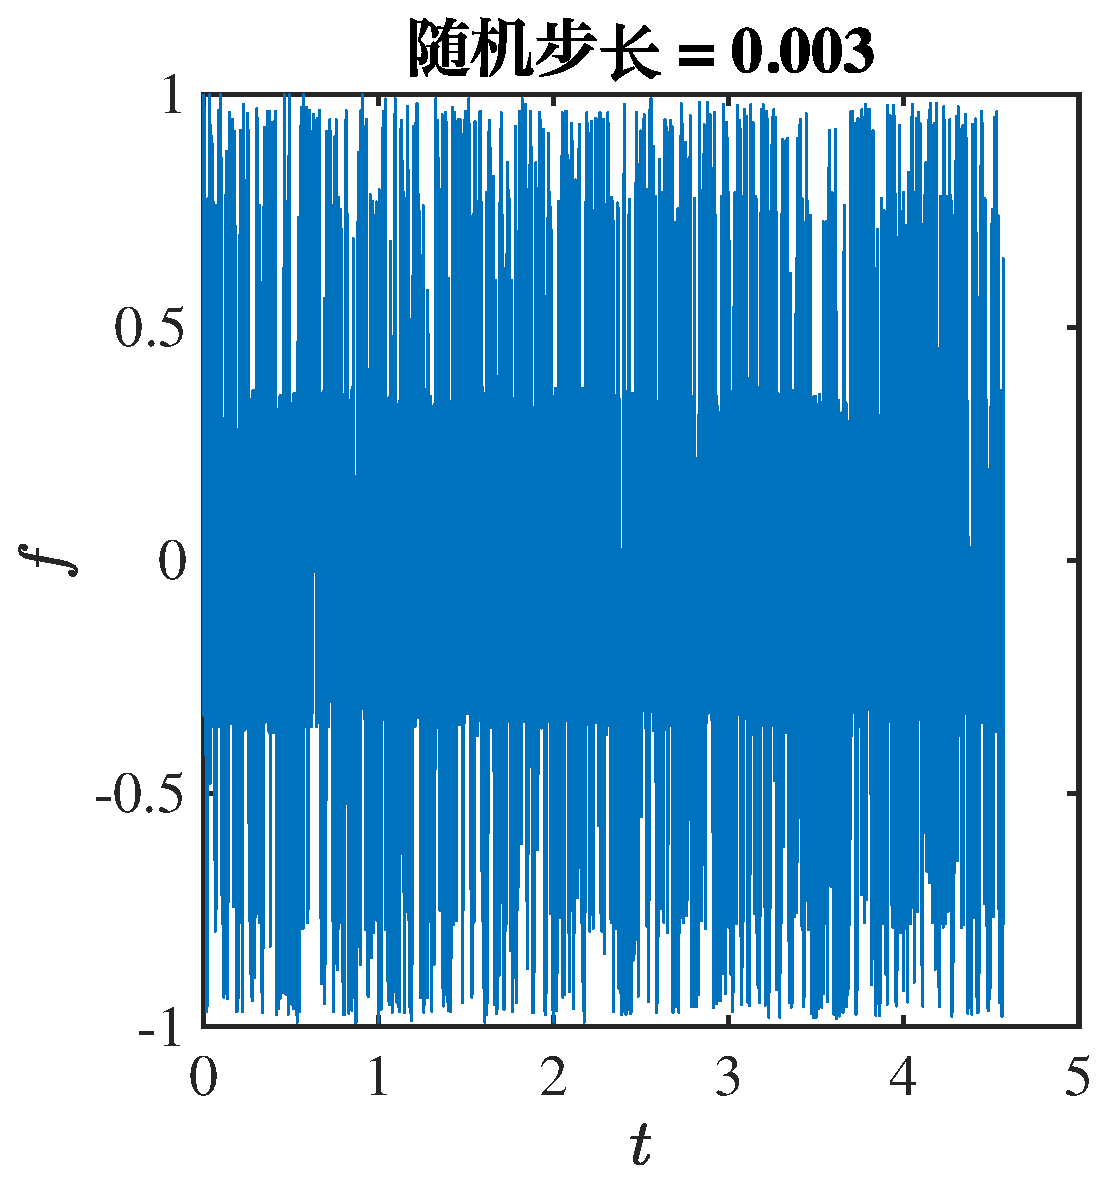
\includegraphics[scale=0.33]{f3e-3L.eps}
	\hspace{0.5in}
	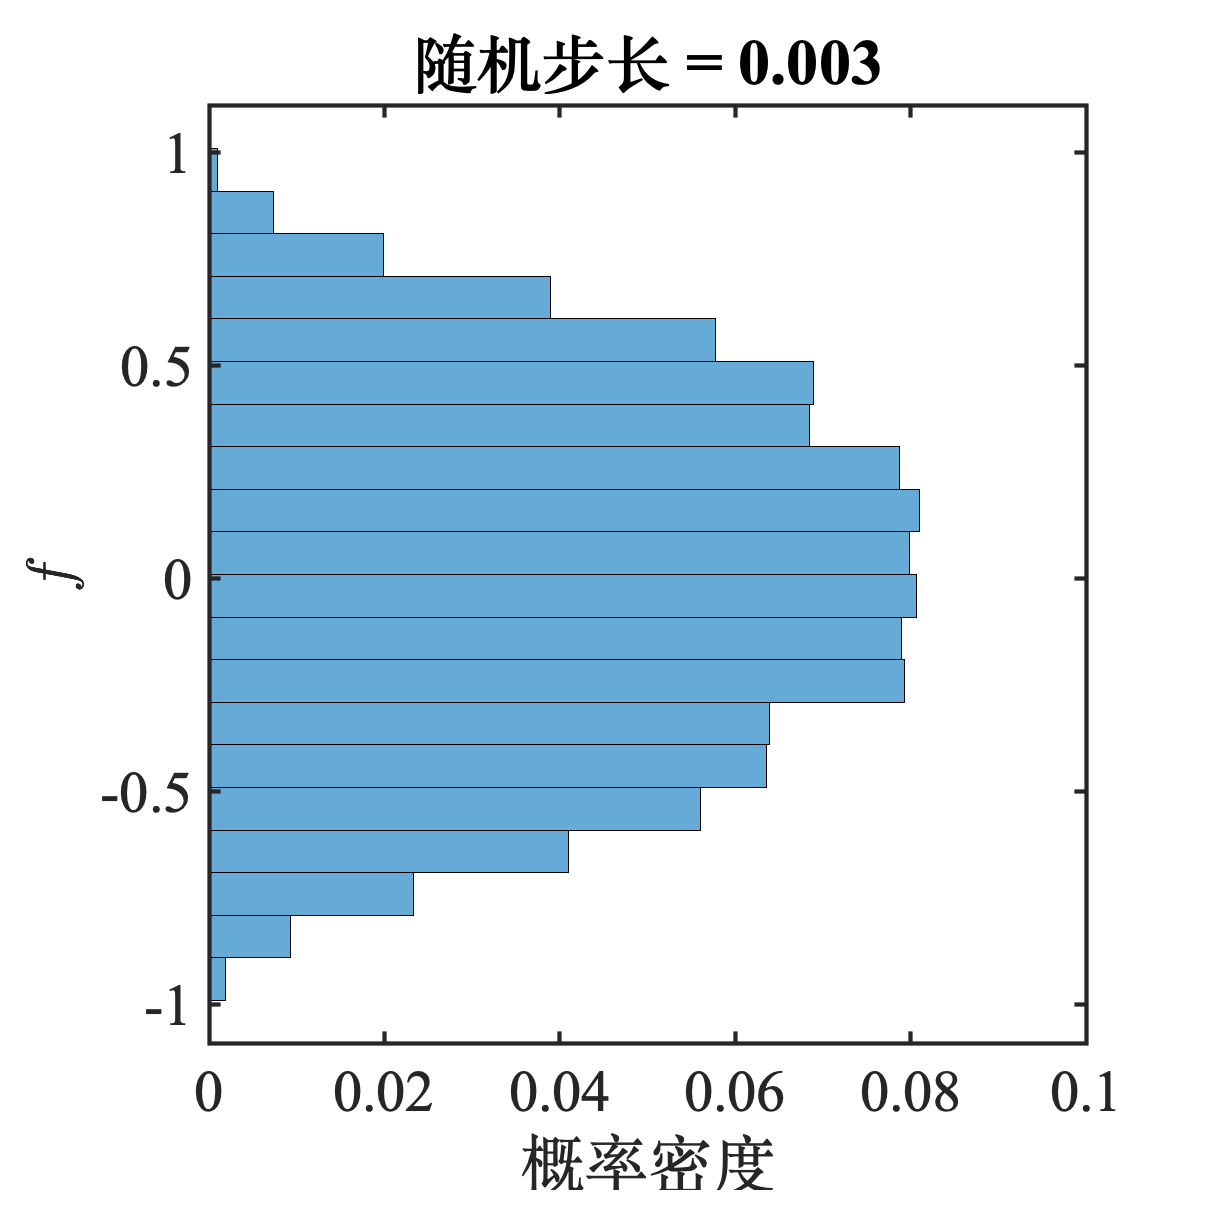
\includegraphics[scale=0.33]{p3e-3L.eps}
	\caption{随机步长$L=0.003$.}
	\label{fig:13e-3}
\end{figure}

\begin{figure}[htp]
	\centering
	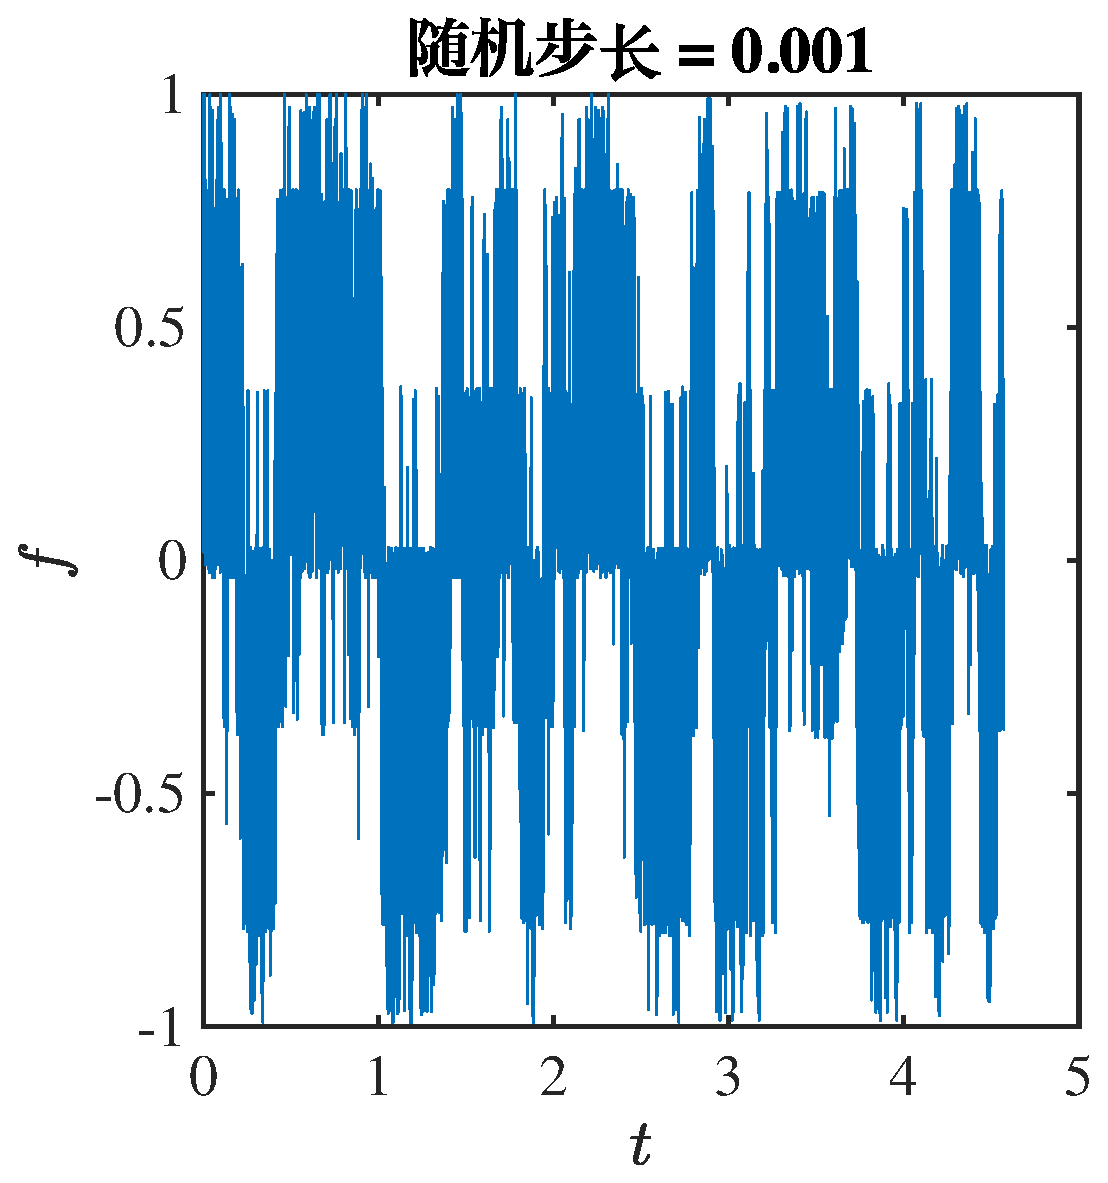
\includegraphics[scale=0.33]{f1e-3L.eps}
	\hspace{0.5in}
	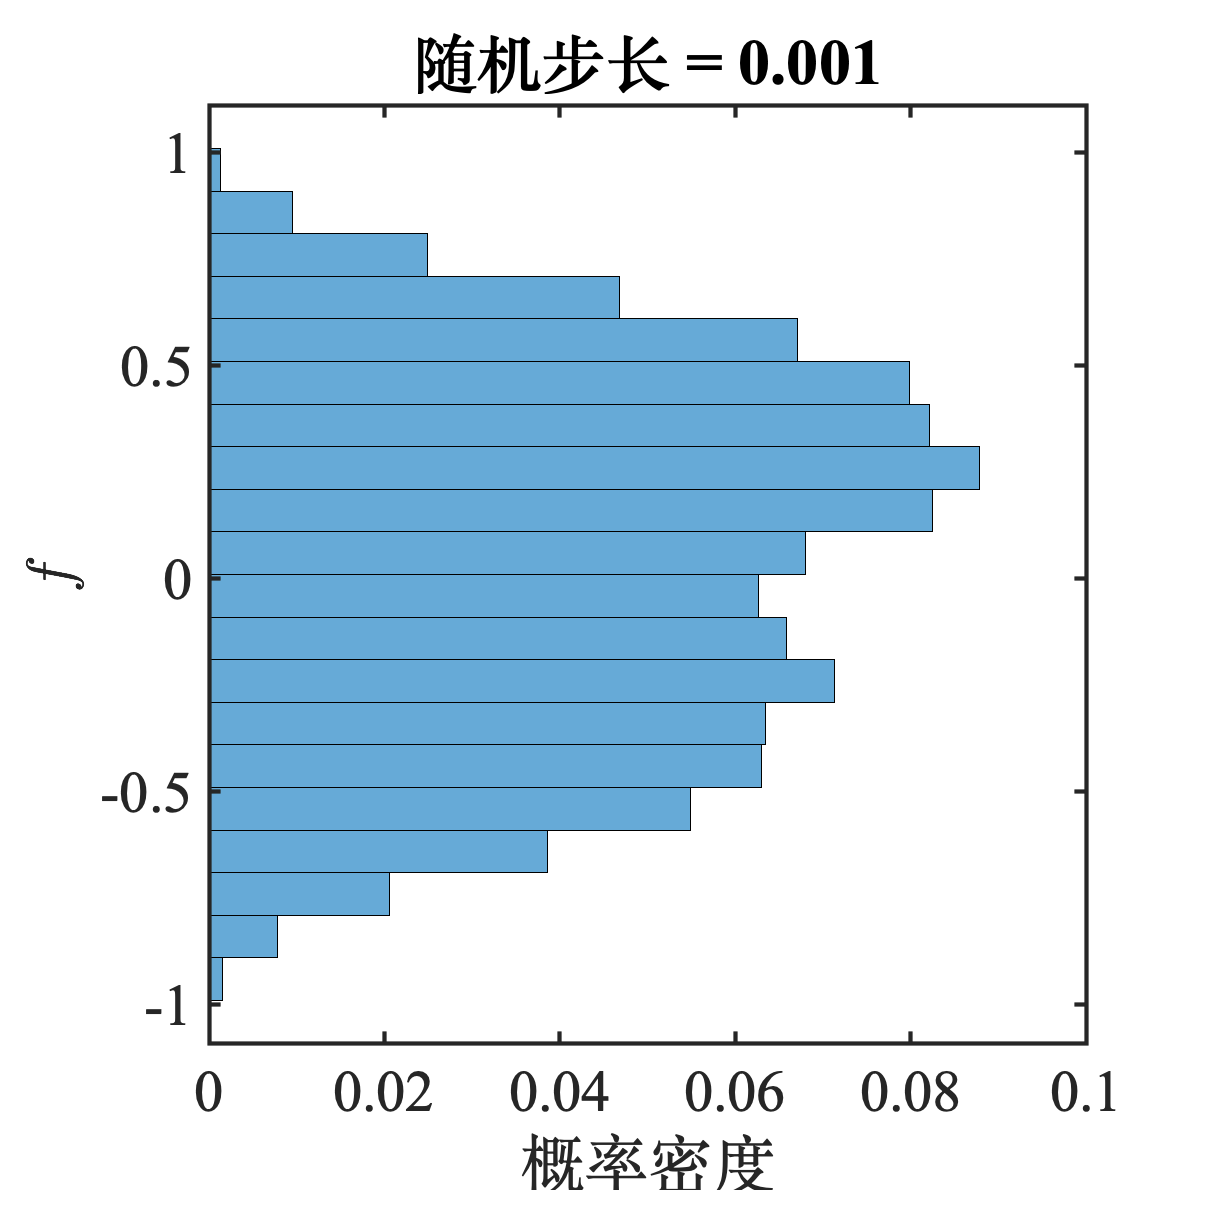
\includegraphics[scale=0.33]{p1e-3L.eps}
	\caption{随机步长$L=0.001$.}
	\label{fig:11e-3}
\end{figure}

二阶结构函数如\cref{fig:1ell1} 所示,可以发现步长不同时,初始值不同,但是前半部分的斜率相同,且最后达到相同的临界值。
\begin{figure}[htp]
	\centering
	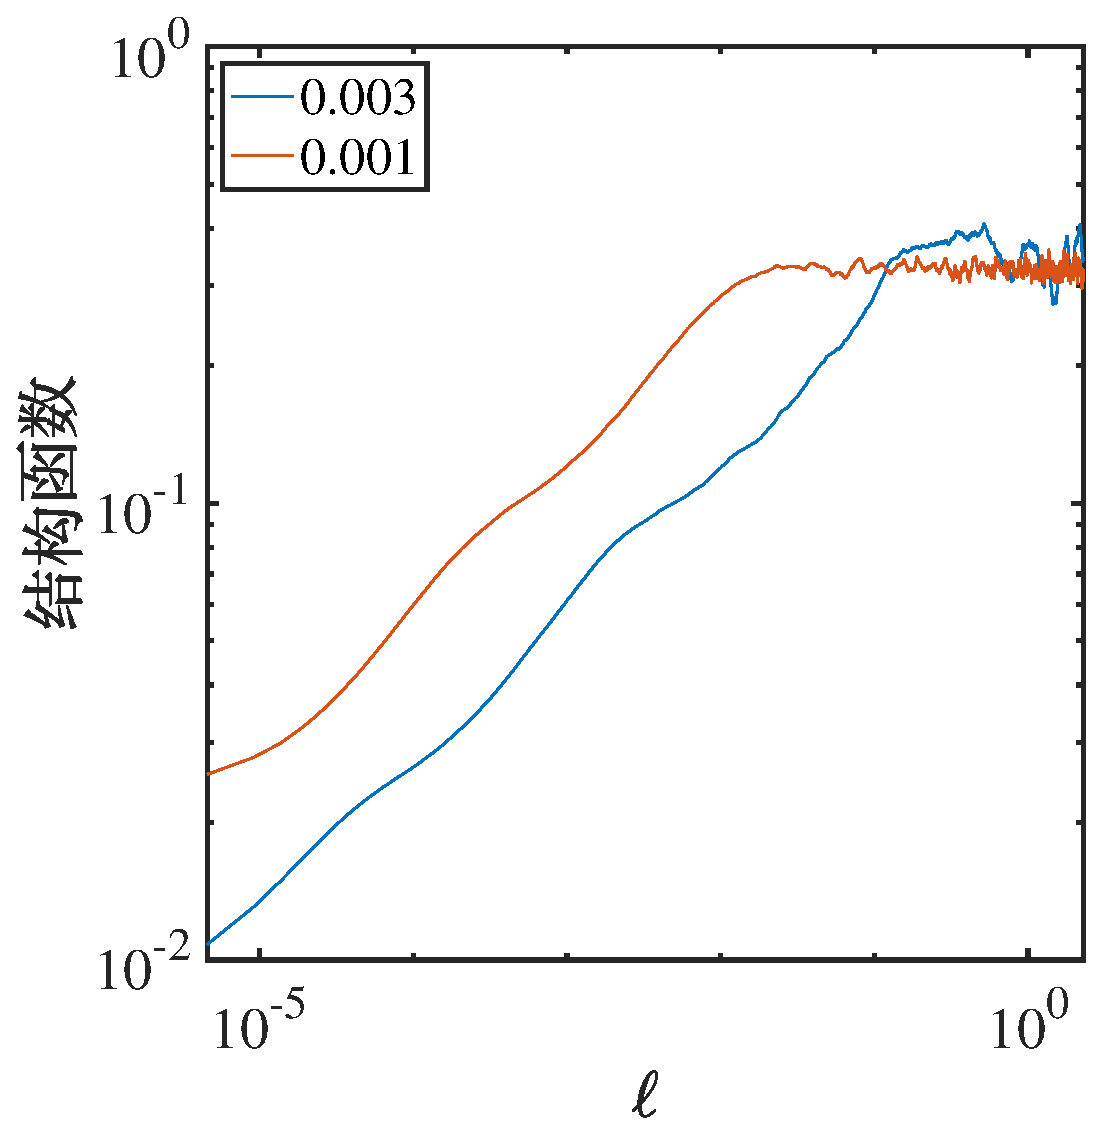
\includegraphics[scale=0.33]{L1e-3L}
	\caption{随机步长$L=0.003$和$L=0.001$.}
	\label{fig:1ell1}
\end{figure}


\section{2}

对于固壁包围的均质不可压缩黏性流体,当容器围绕一个固定不动的轴做刚体旋转时,一定时间后整个容器内的流体都做相对容器静止的刚体运动。可以根据容器尺寸,旋转的角速度和黏性定义一个雷诺数。证明:无论雷诺数多高,容器内流体的这种刚体旋转运动都不会变成湍流。提示:考虑对容器内流体所加扰动(不限于小扰动)的演化。



取相对容器静止的转动柱坐标参考系,容器的转轴和柱坐标的轴重合, N--S方程为
\begin{equation}
	\left\{
	\begin{aligned}
		 & \frac{\partial \bm{v}}{\partial t}+ \bm{v} \cdot \nabla \bm{v} = -\nabla p + \bm{f} + \nu \nabla^2 \bm{v}, \\
		 & \nabla \cdot \bm{v} = 0.
	\end{aligned}
	\right.
\end{equation}
其中$\bm{f}$包括柯氏力和离心力
\begin{equation}
	\bm{f} = \bm{f}_1 + \bm{f}_2 = 2 \bm{\omega} \times \bm{v} + \omega^2\bm{r}.
\end{equation}
其中$\bm{\omega}$是角速度,方向沿转轴,满足右手定则,$\bm{r}$为垂直于转轴,从转轴到物质点的矢量。

下面证明$\bm{f}$不做功。对每一个物质点,科式力垂直于速度,做功功率
\begin{equation}
	p_1 = (2 \bm{\omega} \times \bm{v}) \cdot \bm{v} = 0.
\end{equation}
取任意控制体$V$,功率
\begin{equation}
	\begin{aligned}
		p_2 & =  \int_V \omega^2\bm{r} \cdot \bm{v} \dif v                                                                          \\
		    & =      \frac{1}{2} \omega^2 \int_V \left( \nabla \cdot \left(\bm{v}r^2\right) - r^2 \nabla \cdot \bm{v}\right) \dif v \\
		    & =      \frac{1}{2} \omega^2 \int_V \nabla \cdot \left(\bm{v}r^2\right)  \dif v                                        \\
		    & =      \frac{1}{2} \omega^2 \oiint_S \bm{n} \cdot \left(\bm{v}r^2\right)  \dif s                                      \\
		    & =0.
	\end{aligned}
\end{equation}
其中用到了无散条件和壁面无穿透边界条件。所以只有黏性力做功耗散动能.为了证明动能将趋于$0$,将速度进行螺旋波分解,\cite{yang_su_wu_2010}
\begin{equation}
	\bm{v}=\nabla \phi+\sum_{s} \sum_{\bm{k}} \widehat{v}_{s}(\bm{k}) \bm{\phi}_{s}(\bm{k}, \bm{x}),
	\label{eq:2vhel}
\end{equation}
其中$\{\bm{\phi}_{s}\}$是正交基, $(s,\bm{k})$模态的螺旋波系数是
\begin{equation}
	\widehat{v}_{s}(\boldsymbol{k})=\int_{\mathscr{D}} \boldsymbol{v}(\boldsymbol{x}) \cdot \boldsymbol{\phi}_{s}^{*}(\boldsymbol{k}, \boldsymbol{x}) \mathrm{d} \boldsymbol{x}.
\end{equation}
考虑到边界条件$\bm{v}\big|_{\partial \mathscr{D}}=0$,\cref{eq:2vhel}化为
\begin{equation}
	\bm{v}=\sum_{s} \sum_{\bm{k}} \widehat{v}_{s}(\bm{k}) \bm{\phi}_{s}(\bm{k}, \bm{x}),
	\label{eq:2vhel1}
\end{equation}
对于涡量可以分解为
\begin{equation}
	\bm{\xi}=\nabla \times \boldsymbol{v}=\nabla \varphi+\sum_{s, \boldsymbol{k}}\left[s k \widehat{v}_{s}+b_{s}(\boldsymbol{k})\right] \boldsymbol{\phi}_{s}.
\end{equation}
由于$\bm{v}\big|_{\partial \mathscr{D}}=0$,所以$(\bm{\xi}\cdot \bm{n})\big|_{\partial \mathscr{D}}=0$,上式化为
\begin{equation}
	\bm{\xi}=\sum_{s, \boldsymbol{k}}s k \widehat{v}_{s} \boldsymbol{\phi}_{s}.
\end{equation}

对全场积分得总能量随时间的变化率\cite[P36]{wu_vortical_flows}
\begin{equation}
	\frac{\dif E}{\dif t} = \int_V \rho \frac{\Dif}{\Dif t}\left(\frac{1}{2}v^2\right) \dif V =  \frac{1}{2} \rho \frac{\dif }{\dif t} \int_V v^2 \dif V = -\int_V \Phi \dif V = - \mu  \int_V \xi^2 \dif V.
\end{equation}
将螺旋波分解代入上式可得
\begin{equation}
	\frac{\dif E}{\dif t} = \frac{1}{2} \rho \frac{\dif }{\dif t} \int_V v^2 \dif V =  \frac{1}{2} \rho \frac{\dif }{\dif t} \sum_{s,\bm{k}} \widehat{v}_{s}^2,
\end{equation}
而
\begin{equation}
	\int_V \xi^2 \dif V = \sum_{s, \boldsymbol{k}} k^2 \widehat{v}_{s}^2 \geqslant \sum_{s, \boldsymbol{k}} \widehat{v}_{s}^2,
\end{equation}
所以
\begin{equation}
	\frac{\dif E}{\dif t} = \frac{1}{2} \rho \frac{\dif }{\dif t} \sum_{s,\bm{k}} \widehat{v}_{s}^2 \leqslant - \mu \sum_{s, \boldsymbol{k}}  \widehat{v}_{s}^2.
\end{equation}
由此可见,动能以比指数衰减相等或更快的速度衰减,所以任意的扰动都越来越小,趋于静止,不会发展成湍流。\qed


\section{3}

类似于推导洛伦兹方程的做法,导出两平行平面间热对流的5阶模态满足的常微分方程组,验证该方程组是耗散型的,并问随参数变化有没有混沌现象发生。

推导洛伦兹方程,即:导出两平行平间热对流的3阶模态满足的常微分方程组,验证该方程组是耗散型的。

\textsf{\hspace{-2em}\sf  \textbf{解:}}

\begin{equation}
	\left\{\begin{aligned}
		 & \frac{\partial \nabla^{2} \psi}{\partial t}+\frac{\partial \psi}{\partial x} \frac{\partial \nabla^{2} \psi}{\partial y}-\frac{\partial \psi}{\partial y} \frac{\partial \nabla^{2} \psi}{\partial x}=g \alpha{\frac{\partial \theta}{\partial x}}+ \nu \nabla^{4} \psi, \\
		 & \frac{\partial \theta}{\partial t}+\frac{\partial \psi}{\partial x} \frac{\partial \theta}{\partial y}-\frac{\partial \psi}{\partial y} \frac{\partial \theta}{\partial x} = \frac{\partial \psi}{\partial x} \frac{\Delta T}{d}+\kappa \nabla^{2} \theta.
	\end{aligned}\right.
	\label{eq:31}
\end{equation}
\begin{equation}
	\left\{\begin{array}{l}
		y=0, \psi=\frac{\partial^{2} \psi}{\partial y^{2}}=0, \theta=0, \\
		y=d, \psi=\frac{\partial^{2} \psi}{\partial y^{2}}=0, \theta=0.
	\end{array}\right.
\end{equation}
根据边条件, 采用三角级数展开
\begin{equation}
	\begin{aligned}
		 & \psi(t, x, y)=\sum a_{n m}(t) \sin \left(\frac{n \pi y}{d}\right) \cos \left(\frac{m \pi x}{a}\right)+\sum b_{n m}(t) \sin \left(\frac{n \pi y}{d}\right) \sin \left(\frac{m \pi x}{a}\right),   \\
		 & \theta(t, x, y)=\sum c_{n m}(t) \sin \left(\frac{n \pi y}{d}\right) \cos \left(\frac{m \pi x}{a}\right)+\sum d_{n m}(t) \sin \left(\frac{n \pi y}{d}\right) \sin \left(\frac{m \pi x}{a}\right).
	\end{aligned}
	\label{eq:32}
\end{equation}

将\cref{eq:32}代入\cref{eq:31},并利用三角函数的正交性
\begin{gather}
	\frac{1}{\pi} \int^\pi_{-\pi} \cos mt \cos nt \dif t = \delta_{mn},\\
	\frac{1}{\pi} \int^\pi_{-\pi} \sin mt \sin nt \dif t = \delta_{mn},\\
	\frac{1}{\pi} \int^\pi_{-\pi} \sin mt \cos nt \dif t = 0.
\end{gather}
可得$a_{mn},\, d_{mn} = 0$ 是可能的解,重新定义$a=\pi d/a$,假设题目所说的三阶指的是$m,n \in \{-1,0,1\}$,则$\psi,\theta$的表达式可以写成\cite[P252]{shi}
\begin{equation}
	\pi a \left(\pi^2+a^2\right)^{-1} \kappa^{-1} \psi = X \sqrt{2} \sin \left(\frac{\pi y}{d}\right) \sin \left(\frac{a x}{d}\right),
	\label{eq:33}
\end{equation}
\begin{equation}
	\pi R_c^{-1}R_a \Delta T^{-1} \theta= Y \sqrt{2} \sin \left(\frac{\pi y}{d}\right) \cos \left(\frac{a x}{d}\right)- Z \sin \left(\frac{\pi y}{d}\right).
	\label{eq:34}
\end{equation}
其中$X,\, Y,\, Z.$都只是和无量纲时间$\tau = (\pi^2 + a^2)\kappa t / d^2$有关的函数。 $R_a = g \alpha \Delta T d^3 / (\nu \kappa)$是Rayleigh数, $R_c = (\pi^2+a^2)^3/a^2$是线性化小扰动理论导出的临界Rayleigh数,代入\cref{eq:31}可得
\begin{equation}
	\left\{
	\begin{aligned}
		 & \frac{\mathrm{d} X}{\mathrm{~d} \tau}=-\sigma X+\sigma Y, \\
		 & \frac{\mathrm{d} Y}{\mathrm{~d} \tau}=-X Z+r X-Y,         \\
		 & \frac{\mathrm{d} Z}{\mathrm{~d} \tau}=X Y-b Z.
	\end{aligned}
	\right.
	\label{eq:3lorenz}
\end{equation}
其中 $\sigma=\gamma / \kappa$ 是 Prandtl 数, $r=R_{a} / R_{c},\, b=4\left(1+a^{2} \pi^{-2}\right)^{-1}$ 。此方程组是 Lorenz 方程组。

\cref{eq:3lorenz} 可写成
\begin{equation}
	\frac{\dif \bm{x}}{\dif \tau} = \bm{f},
\end{equation}
其中
\begin{equation}
	\bm{x} = \begin{pmatrix}
		X \\Y\\Z
	\end{pmatrix},\quad
	\bm{f} = \begin{pmatrix}
		-\sigma X+\sigma Y \\-X Z+r X-Y\\X Y-b Z
	\end{pmatrix}.
\end{equation}
设相空间内有一体积$V$,则体积变化
\begin{equation}
	\begin{aligned}
		\frac{\dif V}{\dif \tau} & = \oiint \bm{n} \cdot \bm{f} \dif s                                                                                                                                   \\
		                         & = \int_V \nabla  \cdot \bm{f} \dif v                                                                                                                                  \\
		                         & = \int_V \left(\frac{\partial }{\partial X} (-\sigma X+\sigma Y  ) + \frac{\partial }{\partial Y} (-X Z+r X-Y) + \frac{\partial }{\partial Z} (X Y-b Z )\right)\dif v \\
		                         & = (-\sigma - 1 - b) V.
	\end{aligned}
\end{equation}
由于$-\sigma - 1 - b<0$,所以$V$关于时间指数衰减,所以Lorenz方程组是耗散型的。


\section{4}

证明Chou(1940)中速度4阶关联与2阶关联的准正态分布关系,即:4个独立变量均服从均值为0的正态分布,则下式成立
\begin{equation}
	\left\langle v_{i} v_{j} v_{k} v_{l}\right\rangle=\left\langle v_{i} v_{j}\right\rangle \cdot\left\langle v_{k} v_{l}\right\rangle+\left\langle v_{i} v_{k}\right\rangle \cdot\left\langle v_{j} v_{l}\right\rangle+\left\langle v_{i} v_{l}\right\rangle \cdot\left\langle v_{j} v_{k}\right\rangle.
\end{equation}

提示:参考 \emph{Turbulence, The legacy of A.N.Kolmogorov}.\cite{Frisch_Turbulence}

设中心随机变量$\bm{v} = (v_i,v_j,v_k,v_l)$是高斯分布的,即对任意的 $\bm{c}\in \mathbb{R}^2$,标量$\bm{c}\cdot \bm{v}$是标量高斯随机变量。

高斯分布积分定理:设$\bm{v}$是一个中心向量高斯变量,$f$是$n$变量随机函数,假设所有平均值都存在,则
\begin{equation}
	\left\langle v_i f(v_1,v_2,\ldots,v_n)\right\rangle = \Gamma_{ij} \left\langle \frac{\partial f}{\partial v_j}\right\rangle,
\end{equation}
其中$\Gamma=\left\langle v_i v_j\right\rangle $.

接下来证明
\begin{equation}
	\left.\begin{array}{rl}
		\left\langle v_{i_{1}} v_{i_{2}} \ldots v_{i_{2 m}}\right\rangle= & \sum\left\langle v_{i_{\ell_{1}}} v_{i_{\ell_{2}}}\right\rangle\left\langle v_{i_{\ell_{3}}} v_{i_{\ell_{4}}}\right\rangle \cdots\left\langle  v_{i_{\ell_{2m-1 }}} v_{i_{\ell_{2 m}}}\right\rangle \\
		                                                                  & \forall m, i_{1}, i_{2}, \ldots, i_{2 m}
	\end{array}\right\}
	\label{eq:41}
\end{equation}
其中
\begin{equation}
	\left(\ell_{1}, \ell_{2}\right),\left(\ell_{3}, \ell_{4}\right), \cdots,\left(\ell_{2 m-1}, \ell_{2 m}\right).
\end{equation}
是$\{1,2, \ldots, 2 {m}\}$任意的分割,求和是所有可能的分割。$m=1$时式子很显然成立。假设$m-1$时成立,
\begin{equation}
	\begin{aligned}
		\left\langle v_{i_{1}} v_{i_{2}} \ldots v_{i_{2 m}}\right\rangle & = \left\langle v_{i_{1}} f \right\rangle         \\
		                                                                 & =
		\Gamma_{i_1 j} \left\langle \frac{\partial f}{\partial v_j}\right\rangle                                            \\
		                                                                 & =
		\left\langle v_{i_{1}} v_{j}\right\rangle\left\langle v_{i_{2}} \ldots \hat{v}_{j} \ldots v_{i_{2 m}}\right\rangle. \\
		                                                                 & =
		\sum\left\langle v_{i_{\ell_{1}}} v_{i_{\ell_{2}}}\right\rangle\left\langle v_{i_{\ell_{3}}} v_{i_{\ell_{4}}}\right\rangle \cdots\left\langle  v_{i_{\ell_{2m-1 }}} v_{i_{\ell_{2 m}}}\right\rangle\end{aligned}
\end{equation}
其中$\hat{v}_j$指$v_j$被忽略。上式用到了$m-1$时\cref{eq:41}成立的假设。\qed



\section{5}

证明高雷诺数下射流的耗散率是常数,与粘性无关。

考虑突然扩大管,如\cref{fig:5kuo}
\begin{figure}[htp]
	\centering
	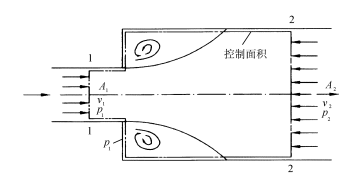
\includegraphics[width=11cm]{kuo.png}
	\caption{突然扩大管.}
	\label{fig:5kuo}
\end{figure}
列出能量
\begin{equation}
	\varepsilon = \left\langle \frac{1}{2} v_1^2 + \frac{p_1}{\rho}\right\rangle - \left\langle \frac{1}{2} v_2^2 + \frac{p_2}{\rho} \right\rangle,
\end{equation}
动量方程
\begin{equation}
	p_1 A_2 - p_2 A_2 = v_2^2 \rho A_2 - v_1^2 \rho A_1,
\end{equation}
质量守恒
\begin{equation}
	A_1 v_1 = A_2 v_2.
\end{equation}

所以
\begin{equation}
	\varepsilon = \left\langle \frac{v_1^2}{2}\right\rangle \left(1-\frac{A_1}{A_2}\right)^2,
\end{equation}
当$A\to +\infty$时即为射流,此时
\begin{equation}
	\varepsilon = \left\langle \frac{v_1^2}{2}\right\rangle
\end{equation}
是常数。\qed









\nocite{*}

% \newpage
\bibliographystyle{plain}
% \clearpage
\phantomsection

\addcontentsline{toc}{section}{参考文献} %向目录中添加条目,以章的名义
\bibliography{homework}

\end{document}
